\section{Framing \& Overlap Add} \label{sec:framing_overlap_add}

The first step, as described in Figure \ref{fig:system}, is the framing of the audio file. This is done according to Equation \ref{eq:framing}. Where $l$ is the frame index (the l-th frame), $n$ is sample number, $R$ is the hoplength. $w[n]$ is the window used to smoothen the signal in such a way that the signal does not become discontinuous and cause wrong sidelobes wen applying the FT.
% N is frame length, R is hoplength, l is frame index.
\begin{equation}
  \label{eq:framing}
  y_{l}[n] = y[n + lR]w[n],\quad n=0,\hdots,N-1
\end{equation}

The last step of the system is the Overlap Add-block. The windowing is removed after which the samples are added back together to one file.
\begin{equation}
  \label{eq:overlap_add}
  y[n] =  \sum_{l=1}^{k} y_{l}[n]/w[n]
\end{equation}

There are various windows that are suited for framing an audio signal. The standard Hamming and Hann window and the square-root Hann window used in a paper by Hendriks\cite{Hendriks} was evaluated. When overlap adding all the frames without applying any changes, the signal should be recovered without any trouble. The overlap added windows should then be equal to an ones vector. Using different values for the overlap percentage, the corresponding overlap add vector is generated and compared to an all-ones vector. An important variable for the framing function is the overlap percentage.  The results in Fig. \ref{fig:opt_oa} show the negative mse of these two vectors. The peak value is around 70\% vor the square-root Hann.

\begin{figure}[h]
  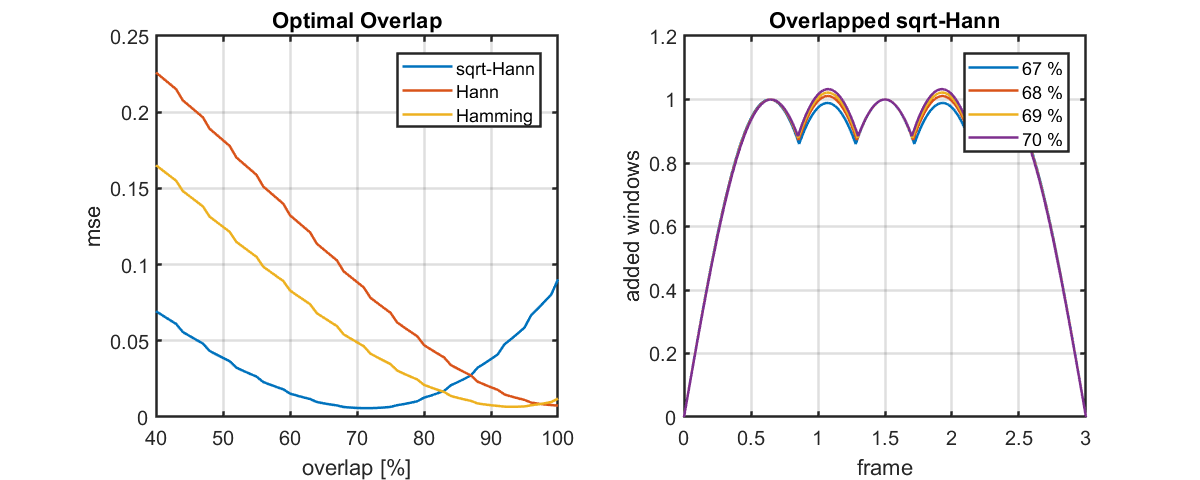
\includegraphics[width=\textwidth]{images/optimal_overlap.png}
  \caption{Optimal overlap percentage for the square-root Hann window.}
  \label{fig:opt_oa}
\end{figure}
